% !TeX spellcheck = en_US
\section{Race Detection by Mining Locking Rules}
\label{sec_technique}
To address the above challenges, we propose three key techniques. For {\em C1}, 
we propose an {\em alias-aware rule mining method} to automatically deduce 
locking rules. For {\em C2}, we propose a {\em lock-usage analysis} to filter 
out false positives caused by kernel code that can not execute concurrently. 
For {\em C3}, we propose a {\em pattern-based estimation} to extract harmful 
data races that can trigger memory or logic bugs such as null-pointer 
dereference, data inconsistencies and double fetches. We introduce them as 
follows:

\subsection{Alias-Aware Rule Mining Method}
\label{subsec_rule_mining}
The relationship between variables and locks is not well documented in OS 
kernels, but it can be inferred from the kernel code. Specifically, a variable 
is often protected by the lock exist in the same data structure. And thus if a 
variable is accessed after acquiring a lock existing in the same data structure 
in most cases, it is likely to be protected by the lock. Whether a variable and 
the protecting lock exist in the same data structure can be determined through 
an alias graph~\cite{Li:ASPLOS22, Kastrinis:CC18}, by finding their common 
ancestor. Based on this insight, we propose an {\em alias-aware rule mining 
method} to deduce locking rules automatically. Moreover, with benefits from 
precise field-sensitive alias relationships of alias graph, our alias-aware 
rule mining method can effectively extract accessed filed and its corresponding 
lock field.

\PP{Alias Graph.} It is an important data structure to infer relationship 
between variable and its protecting lock in our analysis, so we introduce it 
and its update first. 

An alias graph is a 2-tuple $\mathit{G = \left<N, E\right>}$, where 
$\mathit{N}$ is a set of nodes, and each node $\mathit{n}$ represents an alias 
set that points to one abstract object. $\mathit{E}$ is a set of labeled edges. 
Each edge is labeled with a data structure field or a dereference operator 
``$\mathit{*}$'', which represents how an abstract object is accessed. In an 
alias node, a variable residing in a node followed by a sequence of edge
labels forms an access path~\cite{Kastrinis:CC18, Cheng:PLDI00}. In this paper, 
we replace the variable in an access path with its structure name to represent 
a data structure field.

An alias graph is updated by handling four types of instructions that  
change alias relationships: MOVE($\mathit{v_1 = v_2}$), STORE ($\mathit{*v_2 = 
v_1}$), LOAD ($\mathit{v_1 = *v_2}$) and GEP ({$\mathit{v_1 = \&v_1->f}$}). We 
exploit {$\mathit{n_x}$} to represent the node whose representing alias set 
includes $\mathit{v_x}$, and introduce how the four types of instructions 
update alias graphs. For a MOVE operation, $\mathit{v_1}$ is moved from 
$\mathit{n_1}$ to $\mathit{n_2}$. After this operation, $\mathit{v_1}$ and  
$\mathit{v_2}$ are represented by the same node, which indicates they become 
aliases. For a STORE operation, the existing outgoing edge from $\mathit{n_2}$ 
is dropped first, and then a new edge labeled with $\mathit{*}$ from 
$\mathit{n_2}$ to $\mathit{n_1}$ is inserted. After this operation, 
$\mathit{v_1}$ and $\mathit{*v_2}$ are represented by the same node, which 
indicates they become aliases. For a LOAD operation, the analysis first finds 
the destination node of the edge that comes from $\mathit{n_2}$ and is labeled 
with $\mathit{*}$, and then moves $\mathit{v_1}$ to the destination node. And 
after this operation, $\mathit{v_1}$ and $\mathit{*v_2}$ are represented by the 
same node, which indicates they become aliases. GEP operation is similar to 
LOAD, expect that the edge is labeled with a data structure field $\mathit{f}$, 
instead of a dereference operator $\mathit{*}$.

\begin{figure}[htbp]
	\centering
	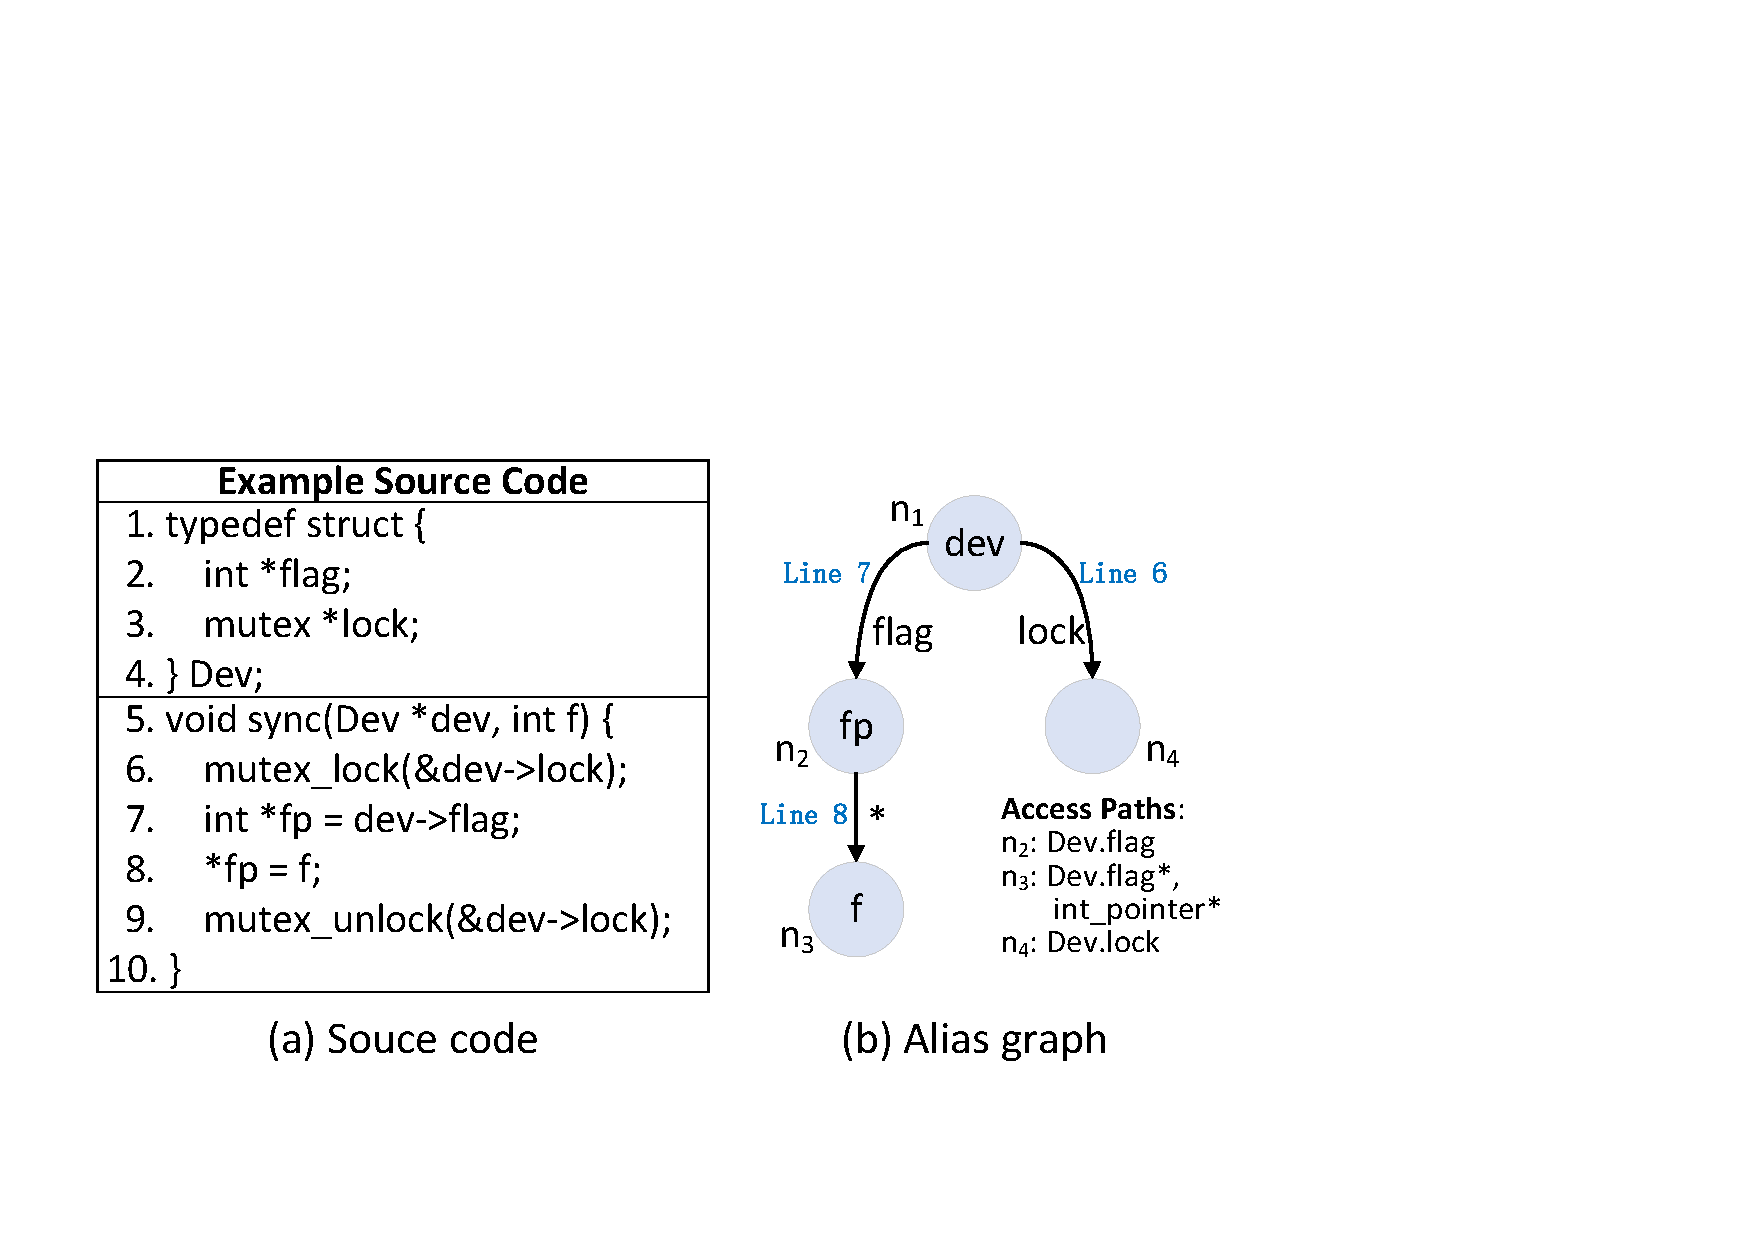
\includegraphics[width=0.9\linewidth]{figures/fig_demo_alias_graph.pdf}
	\figcaption{Example of alias graph.}
	\label{fig_demo_alias_graph}
\end{figure}

\noindent{\textbf{\em Example.}} Figure~\ref{fig_demo_alias_graph} shows a 
piece of driver-like source code and its alias graph. In this example, after a 
GEP (\&dev->lock) operation at Line 6, an edge labeled with {\tt lock} from 
node $\mathit{n_1}$ to node $\mathit{n_4}$ is inserted. Similarly, an edge 
labeled with {\tt flag} from node $\mathit{n_1}$ to node $\mathit{n_2}$ is 
inserted after Line 7. At last, an edge labeled with a dereference operator 
($\mathit{*}$) is inserted after the STORE (*fp = f) operation at Line 8. The 
final alias graph is shown in Figure~\ref{fig_demo_alias_graph}(b), and access 
paths are shown in the bottom left corner. Take node $\mathit{n_3}$ as an 
example, it can represent two fields, one is {\tt Dev.flag*}, and the other is 
{\tt int\_pointer*} (we exploit int\_pointer to represent a pointer points to 
an integer, and regard it as a data structure for convenience). 

\begin{figure}[htbp]
	\centering
	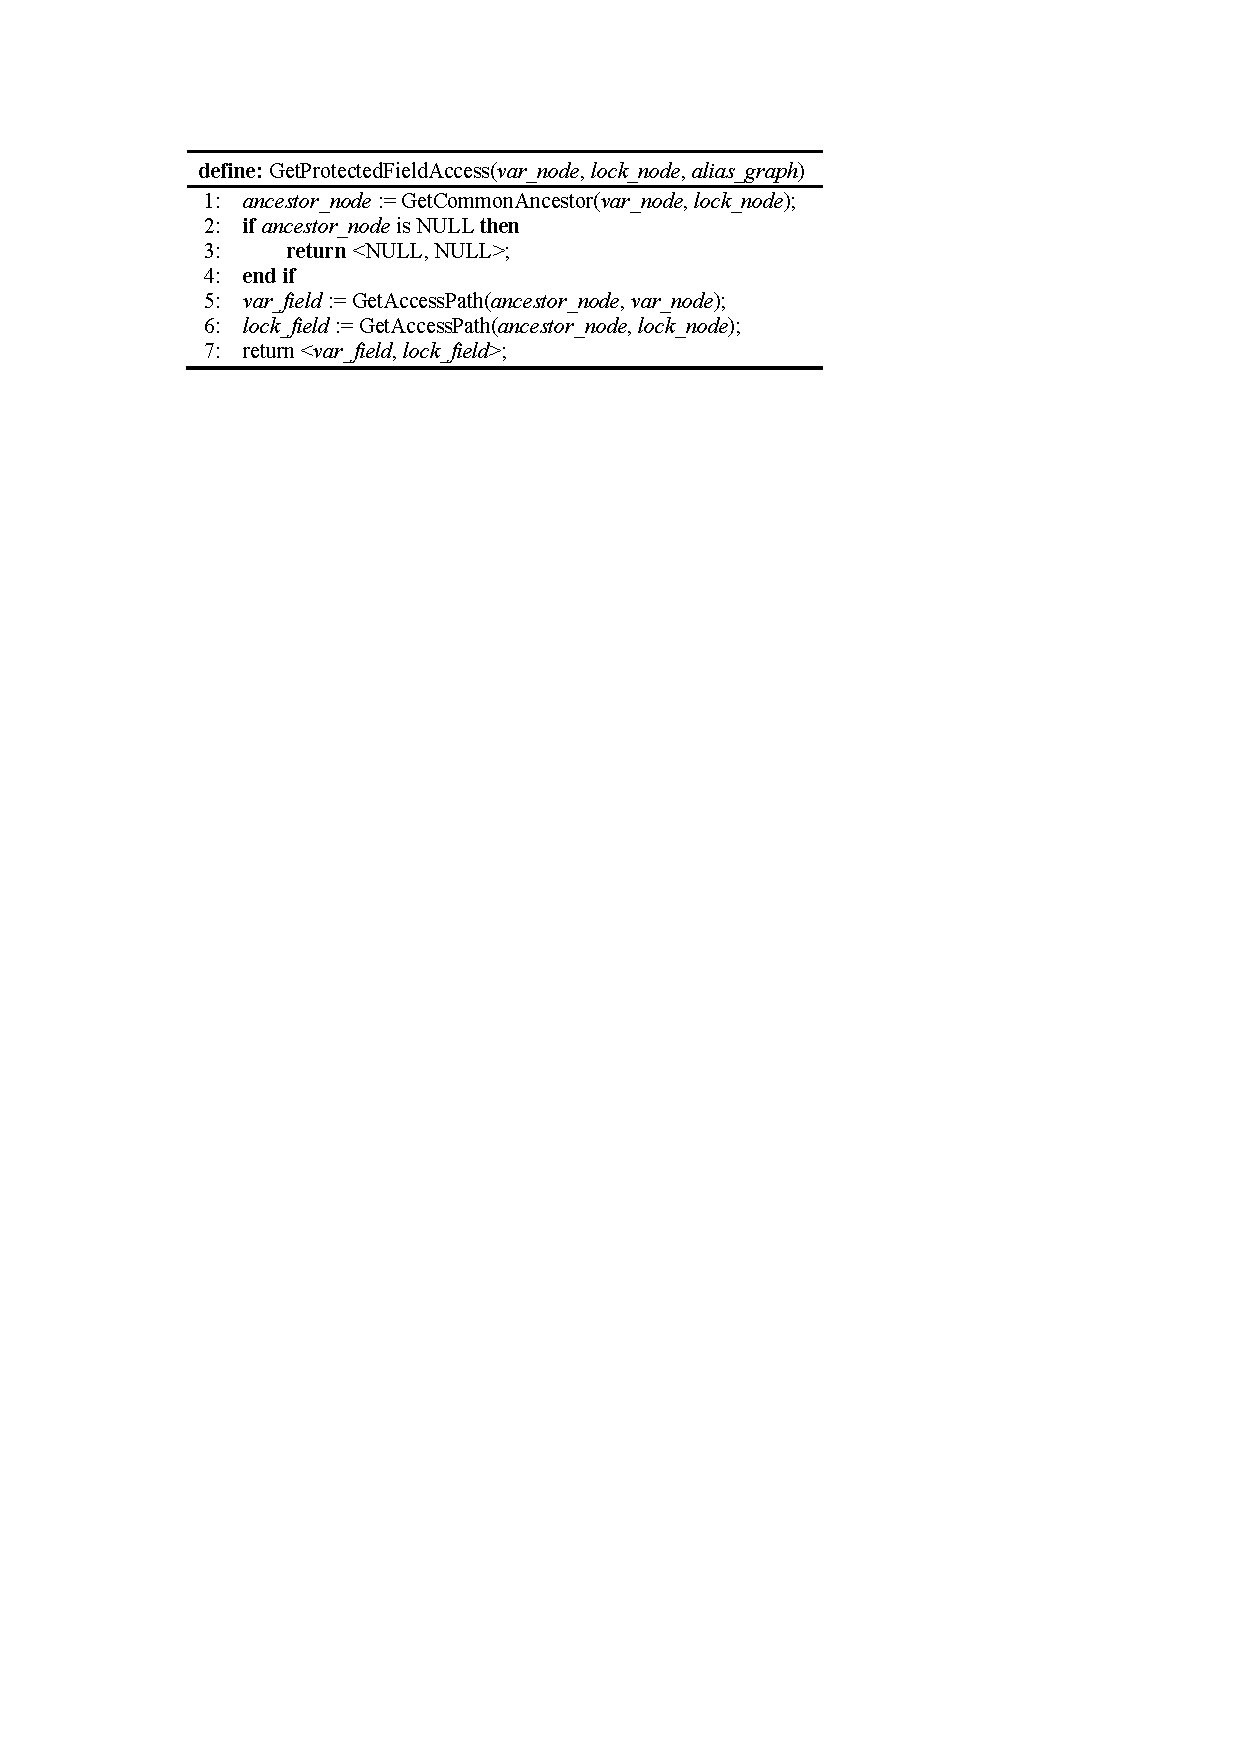
\includegraphics[width=1\linewidth]{figures/fig_pseudocode_get_access.pdf}
	\figcaption{Pseudocodes to get accessed field and protecting lock.}
	\label{fig_pseudocode_get_access}
\end{figure}

Given an alias graph, whether a variable and a lock exist in the same data 
structure can be determined by finding a common ancestor. If they are in the 
same data structure, the variable is likely to be protected by the lock. 
Figure~\ref{fig_pseudocode_get_access} shows the pseudocode to 
get the field of the accessed variable and the field of the protecting lock in 
the form of access path, if they exist in the same data structure. Given a node 
of an accessed variable and a node of a lock variable, the analysis first gets 
the common ancestor of the two nodes (Line 1). And then, if the common ancestor 
does not exist, the analysis returns a NULL pair (Lines 2-3). Otherwise, the 
analysis gets the access paths for the node of the accessed variable and the 
node of the protecting lock from the common ancestor (Lines 5-7).

Take the alias graph in Figure~\ref{fig_demo_alias_graph} as an example, the 
accessed variable {\tt dev->flag} is represented by node $\mathit{n_2}$, and 
the lock {\tt dev->lock} is represented by node $\mathit{n_4}$. The two nodes 
have a common ancestor $\mathit{n_1}$, and thus the accessed variable {\tt 
dev->flag} and the lock {\tt dev->lock} can be inferred to exist in the same 
data structure (namely {\tt Dev}). Therefore, the structure field Dev.flag is 
likely to be protected by the lock stored in the structure field Dev.lock.

\begin{figure}[htbp]
	\centering
	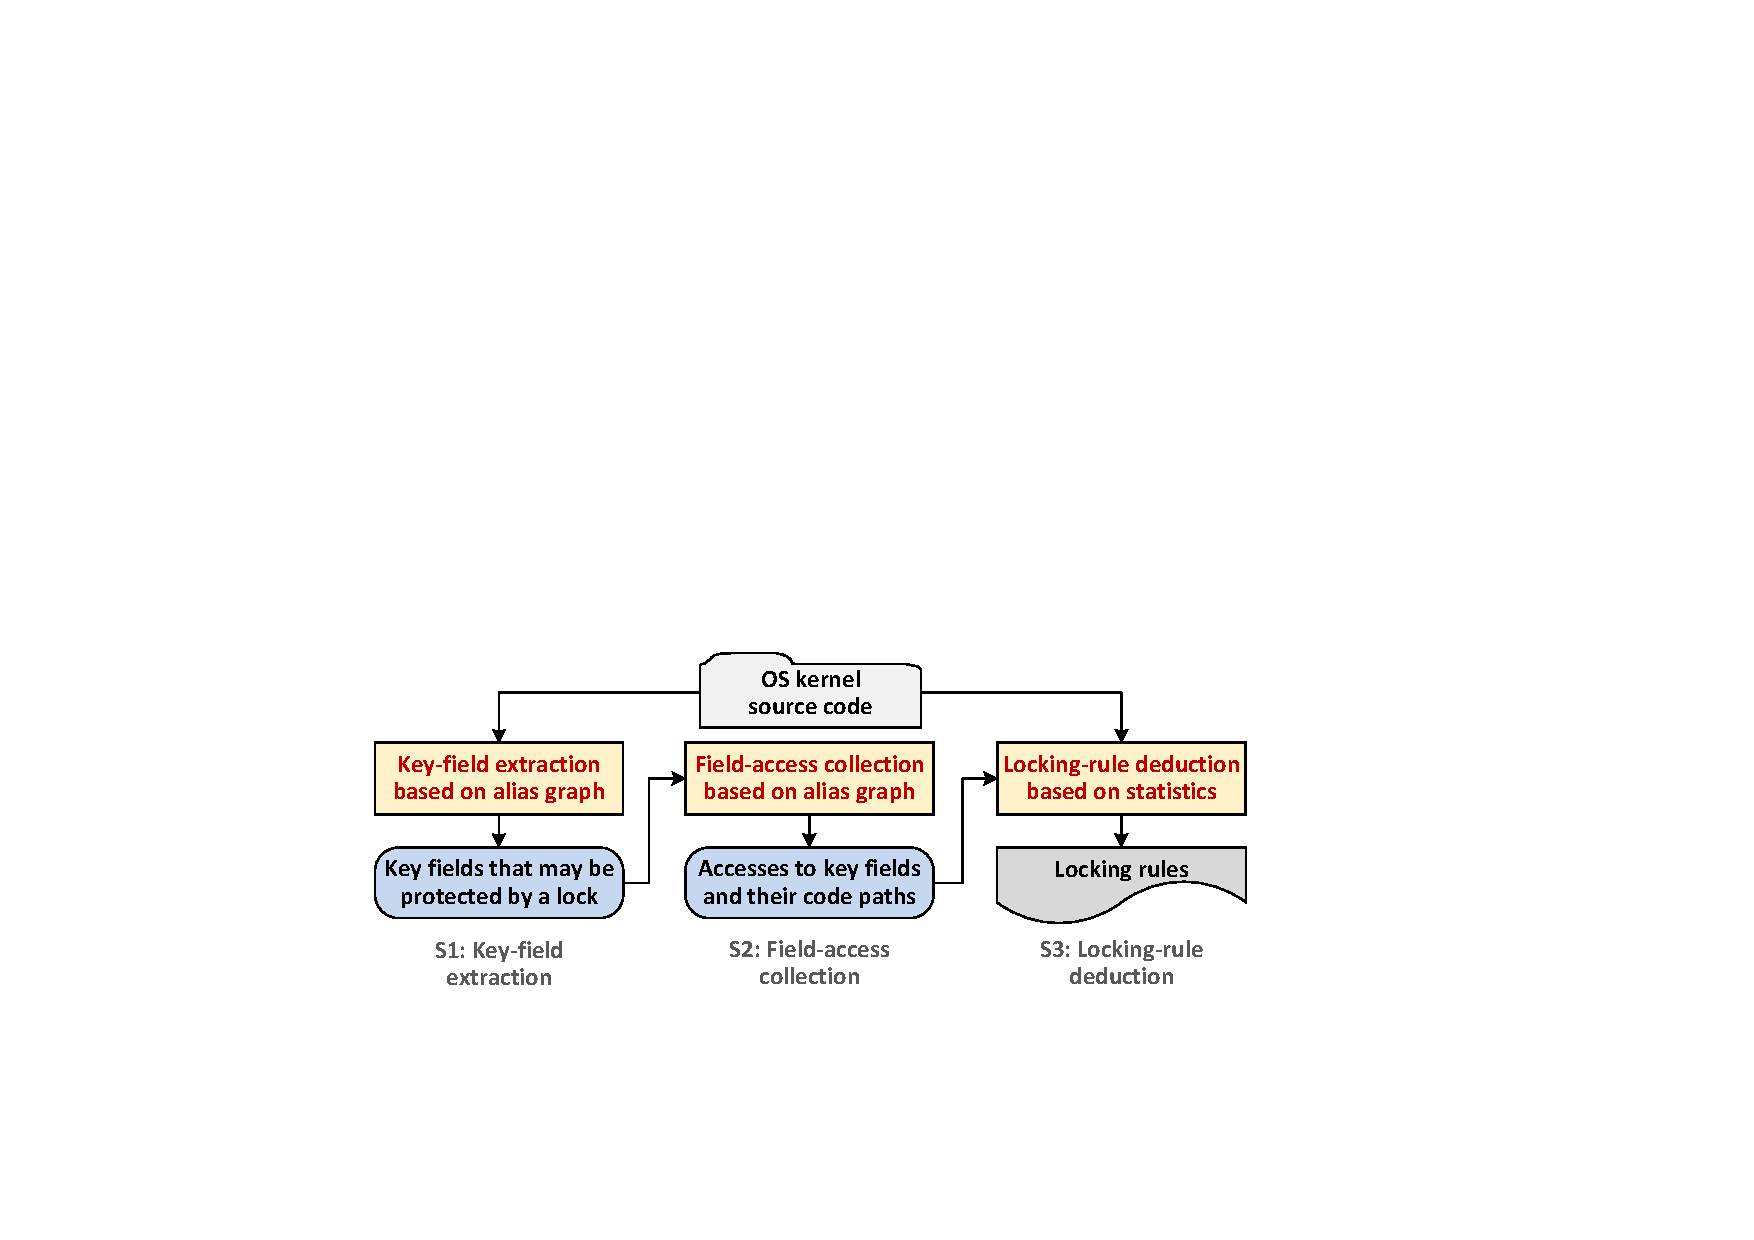
\includegraphics[width=1\linewidth]{figures/fig_workflow.pdf}
	\figcaption{Workflow of locking-rule mining.}
	\label{fig_workflow}
\end{figure}

Based on the alias graph, our alias-aware rule mining method performs an 
inter-procedural, path-based~\cite{Li:ASPLOS22}, field-sensitive and 
alias-aware analysis to effectively mine locking rules about whether accesses 
to a specific data structure field should be protected and which data structure 
field the protecting lock exist in. Overall, our alias-aware rule mining method 
has three main stages shown in Figure~\ref{fig_workflow}. In Stage 1, it 
extracts key fields that may be protected by a lock. In Stage 2, it collects 
all accesses to key fields as well as code paths these accesses exist in. In 
Stage 3, it deduces locking rules by calculating the proportion of field 
accesses protected by a specific lock in all field accesses. 

\PP{S1: Key-field extraction.} The OS kernel has a large code base with 
numerous variables. However, only a small part of variables should be protected 
by a specific lock, and thus collecting all variable accesses can introduce 
much unnecessary overhead. Generally, given a data structure field, only a 
small portion of accesses to it can miss necessary protecting locks, due to the 
carelessness of developers. Based on this insight, our analysis first extracts 
key fields that may need to be protected by a specific lock, by performing a 
lock-set analysis to find whether a given variable is accessed after acquiring 
a lock in the same data structure in any code path.

\begin{figure}[htbp]
	\centering
	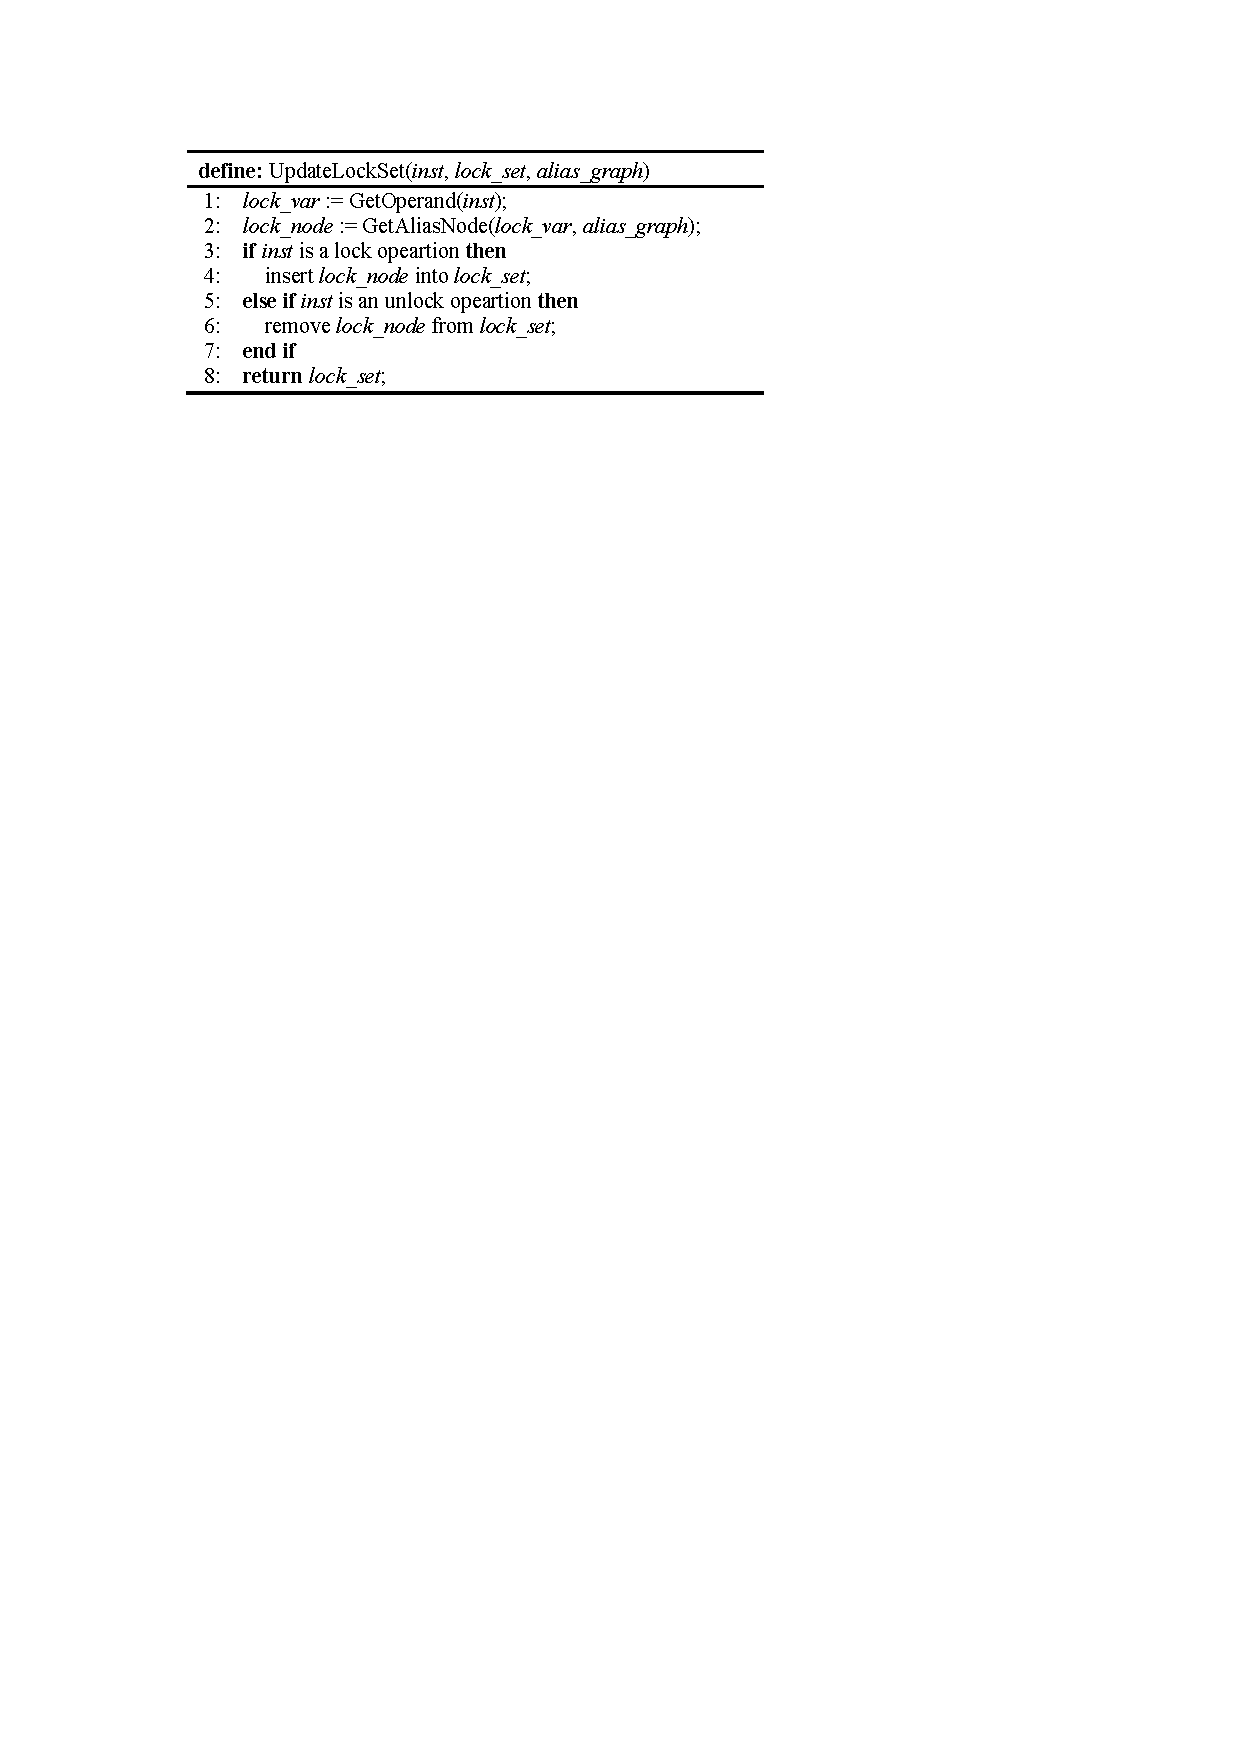
\includegraphics[width=1\linewidth]{figures/fig_pseudocode_lock_set.pdf}
	\figcaption{Pseudocodes of lock-set analysis.}
	\label{fig_pseudocode_lock_set}
\end{figure}

Figure~\ref{fig_pseudocode_lock_set} shows the lock-set analysis based on alias 
graph. The analysis first gets the operand of the instruction (Line 1), and 
then gets the node of the operand from the alias graph (Line 2). If the 
instruction is a lock operation, the node of the operand is inserted into the 
lock set, which stores all nodes of the acquired locks (Lines 3-4). Otherwise, 
if the instruction is an unlock operation, the node of the operand is removed 
from the lock set (Lines 5-6).

\begin{figure}[htbp]
	\centering
	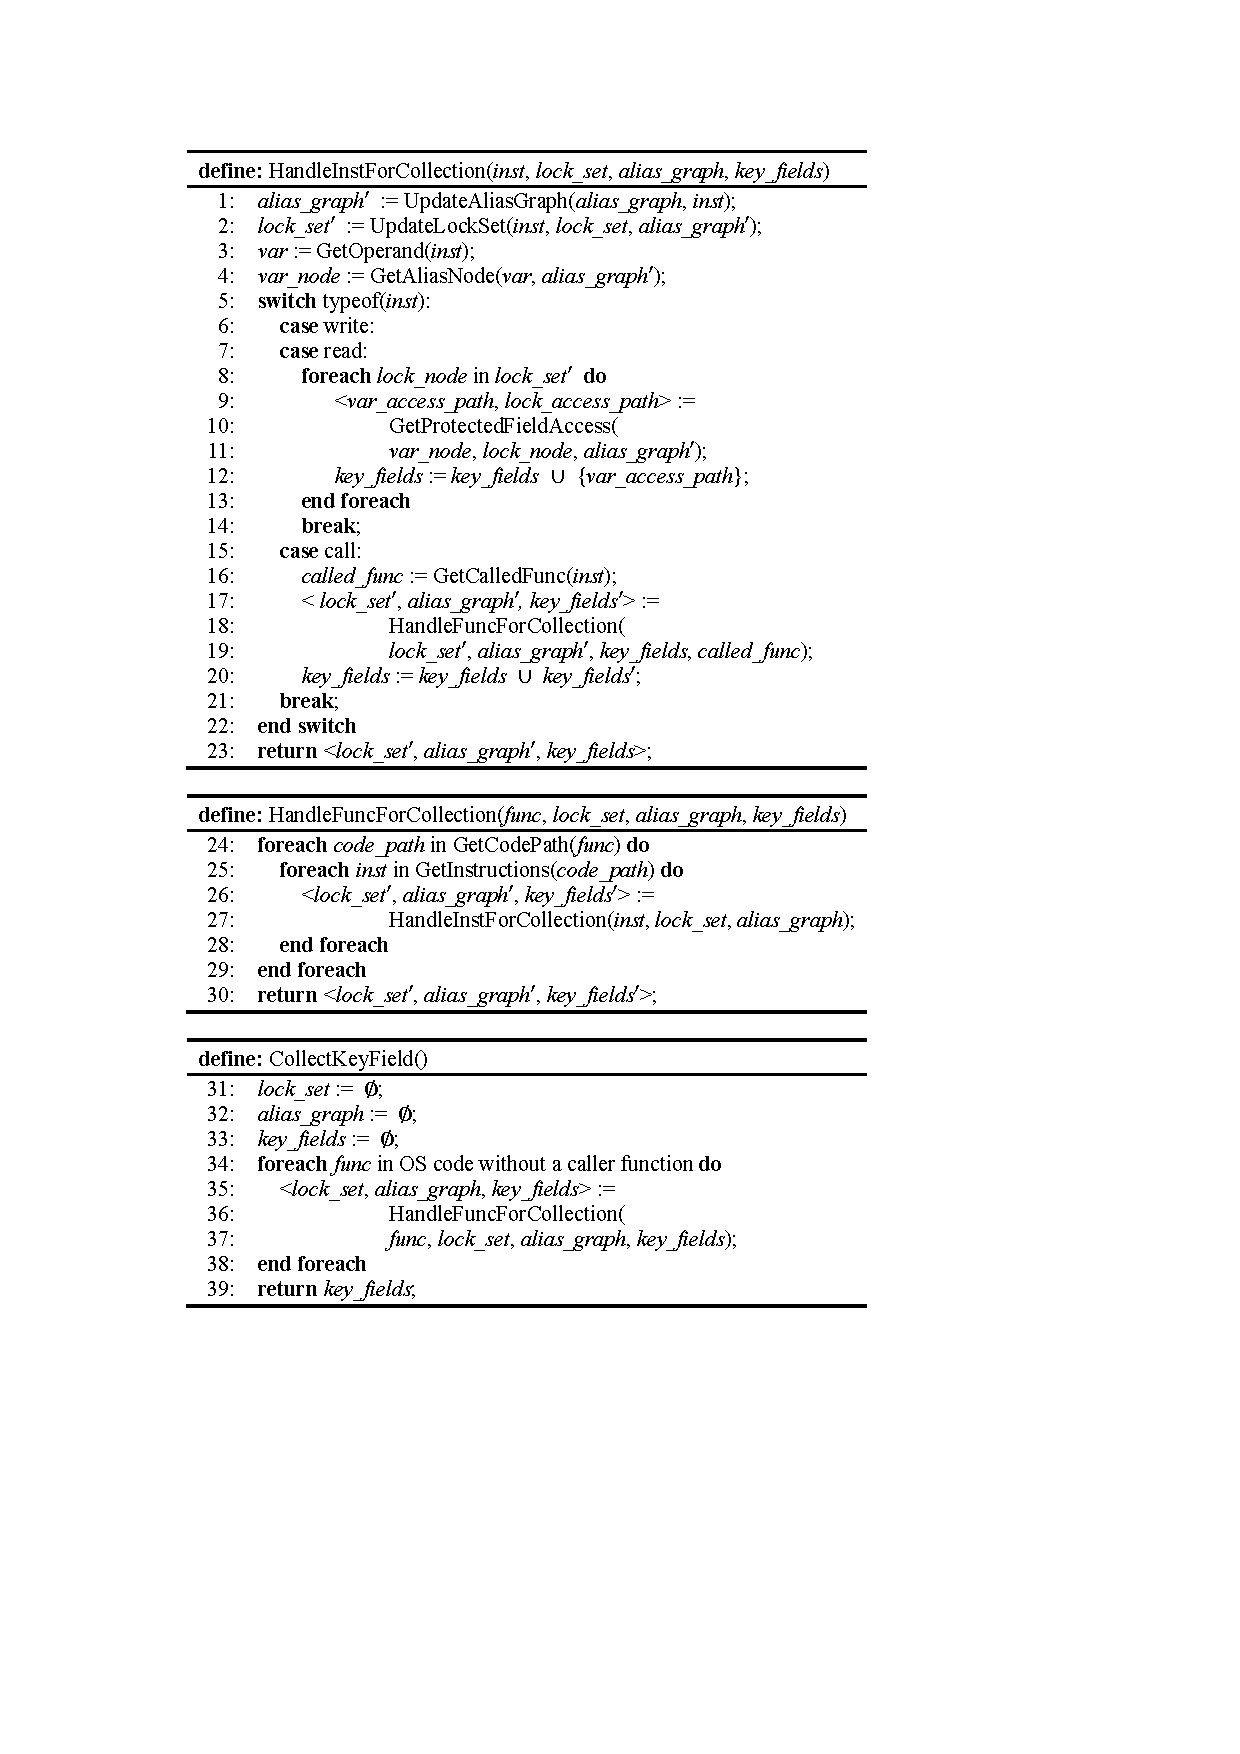
\includegraphics[width=1\linewidth]{figures/fig_pseudocode_field_extract.pdf}
	\figcaption{Pseudocodes of key-field extraction.}
	\label{fig_pseudocode_field_extract}
\end{figure}

Figure~\ref{fig_pseudocode_field_extract} shows the pseudocode to extract key 
fields that may be protected by a specific lock, based on the lock-set analysis 
and the alias graph. The analysis starts from each function without a caller 
function (Lines 16-26) and performs a path-based analysis~\cite{Li:ASPLOS22} 
(Lines 17-25). For each instruction in the code path, the analysis first 
updates the alias graph according to the instruction with the four operations 
(MOVE, STORE, LOAD and GEP) that can change alias relationships (Line 1), and 
then performs a lock-set analysis (Line 2) to get all acquired locks. After 
updating the alias graph and the lock set, if the instruction is a write or a 
read, the analysis first gets the node of the operand with the new alias graph 
(Lines 4-5). And then, for each node of the acquired lock in the lock set, the 
analysis uses the alias graph to extract the protected data structure field 
(Lines 6-12). If the field is not NULL, it is inserted into the set of key 
fields (Lines 9-11). Note that to perform inter-procedural analysis, the 
analysis copies each function definition into its call sites, but this 
operation is not shown in Figure~\ref{fig_pseudocode_field_extract} for 
convenience. 

\PP{S2: Field-access collection.} With the key fields extracted in Stage 1, the 
analysis only needs to collect accesses to the data structure field that are 
protected in some cases, because if a field is never protected by any lock when 
is accessed, it is less likely to be shared by different threads, and thus can 
not introduce any concurrency issue.

\begin{figure}[htbp]
	\centering
	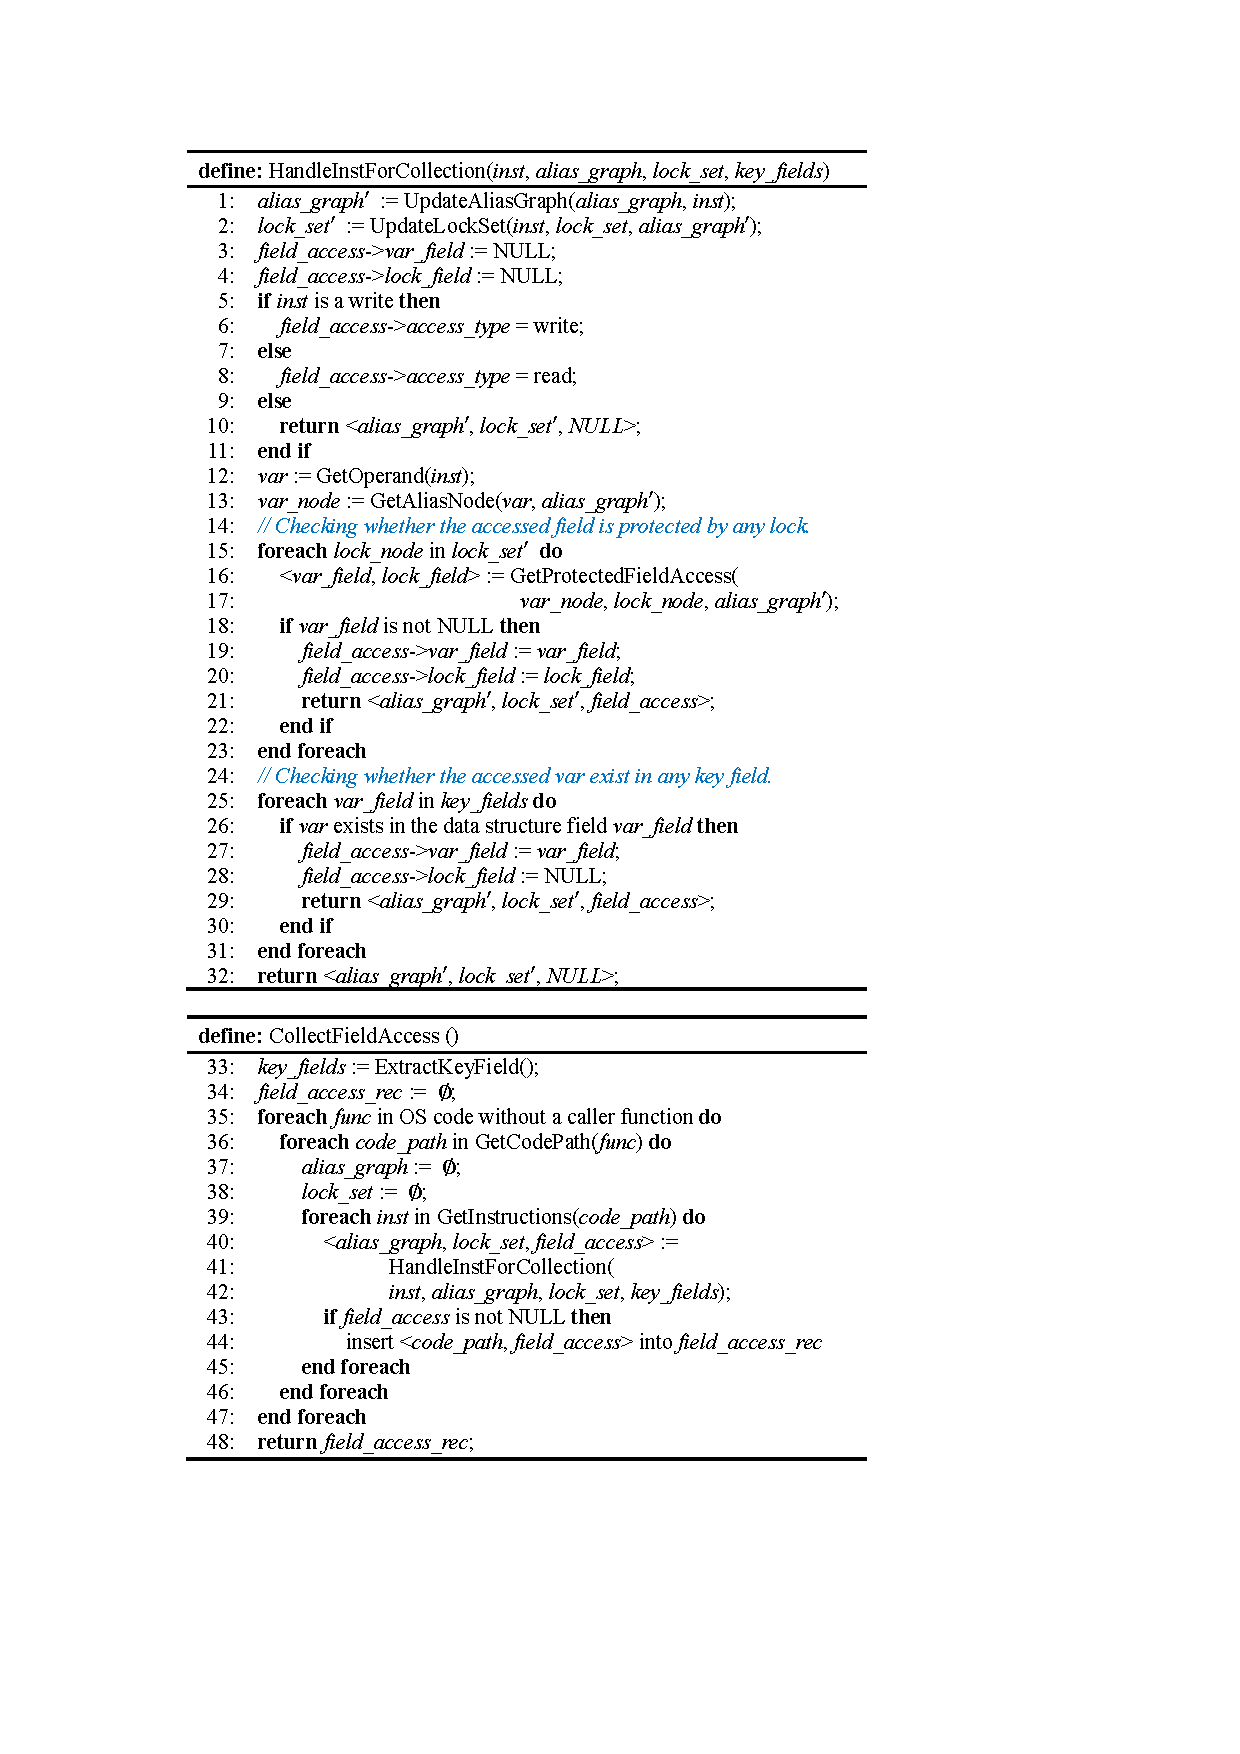
\includegraphics[width=1\linewidth]{figures/fig_pseudocode_access_collect.pdf}
	\figcaption{Pseudocodes of field-access collection.}
	\label{fig_pseudocode_access_collect}
\end{figure}

Figure~\ref{fig_pseudocode_access_collect} shows the pseudocode to collect all 
accesses to key fields. Similarly to the key-field extraction, this stage also 
performs a path-based analysis. For each instruction in the code path (Lines 
39-45), the analysis first updates the alias graph and the lock set according 
to the handled instruction (Lines 1-2). And then, the access type (either a 
write or a read) of a field access is set according to the instruction (Lines 
5-8). However, if the instruction is not an access operation, the function 
returns a NULL value for the field access (Line 10). Otherwise, the analysis 
first gets the node of the operand with the new alias graph (Lines 12-13), and 
then for each node of the acquired lock in the lock set, the analysis uses the 
alias graph to extract the fields that the accessed variable and the acquired 
lock stored in (Lines 16-17). If the fields are found, the field access is 
returned with the found fields (Lines 18-22). Otherwise, the accessed field is 
not protected by any lock. In this case, if the accessed variable is stored in 
a key field, the field access is returned with a NULL lock (Lines 25-30).

\PP{S3: Locking-rule deduction.} After collecting all accesses to key fields, 
the analysis deduces locking rules based on statistics. However, on the one 
hand, distinguishing different accesses to the same data structure field by 
different program sites is not fine-grained enough, because the access to a 
field and the acquirement to a specific lock are often packaged in a special 
function, and all accesses under different calling context are regarded as the 
same access in this strategy. On the other hand, distinguishing accesses by 
different code paths can also suffer from inaccuracy when a function contains 
many branch statements, because accesses to the same field is regarded as 
different in different code paths, causing numerous accesses to the same field 
due to large quantities of code paths. Based on this consideration, the 
analysis distinguishes accesses to the same data structure field by different 
calling contexts. Specifically, given a key field {\em f} and a lock {\em l}, 
the analysis first finds all access to {\em f} with lock {\em l} from the 
collected field accesses in Stage 2, and gets the number {\em 
locked\_access\_num} by counting different calling contexts extracted from the 
code paths of these field accesses. Then, the analysis finds all access to {\em 
f} (no matter whether a lock is held), and gets the number {\em 
all\_access\_num} in the same way as {\em locked\_access\_num}. If the ratio 
{\em locked\_access\_num} / {\em all\_access\_num} is larger than a given 
threshold, and there is at least one write access to {\em f}, the data 
structure field {\em f} is inferred to be protected by the lock {\em l}. After 
deducting locking rules, the analysis detects data races by checking whether a 
field access validates any locking rules.

\begin{figure}[htbp]
	\centering
	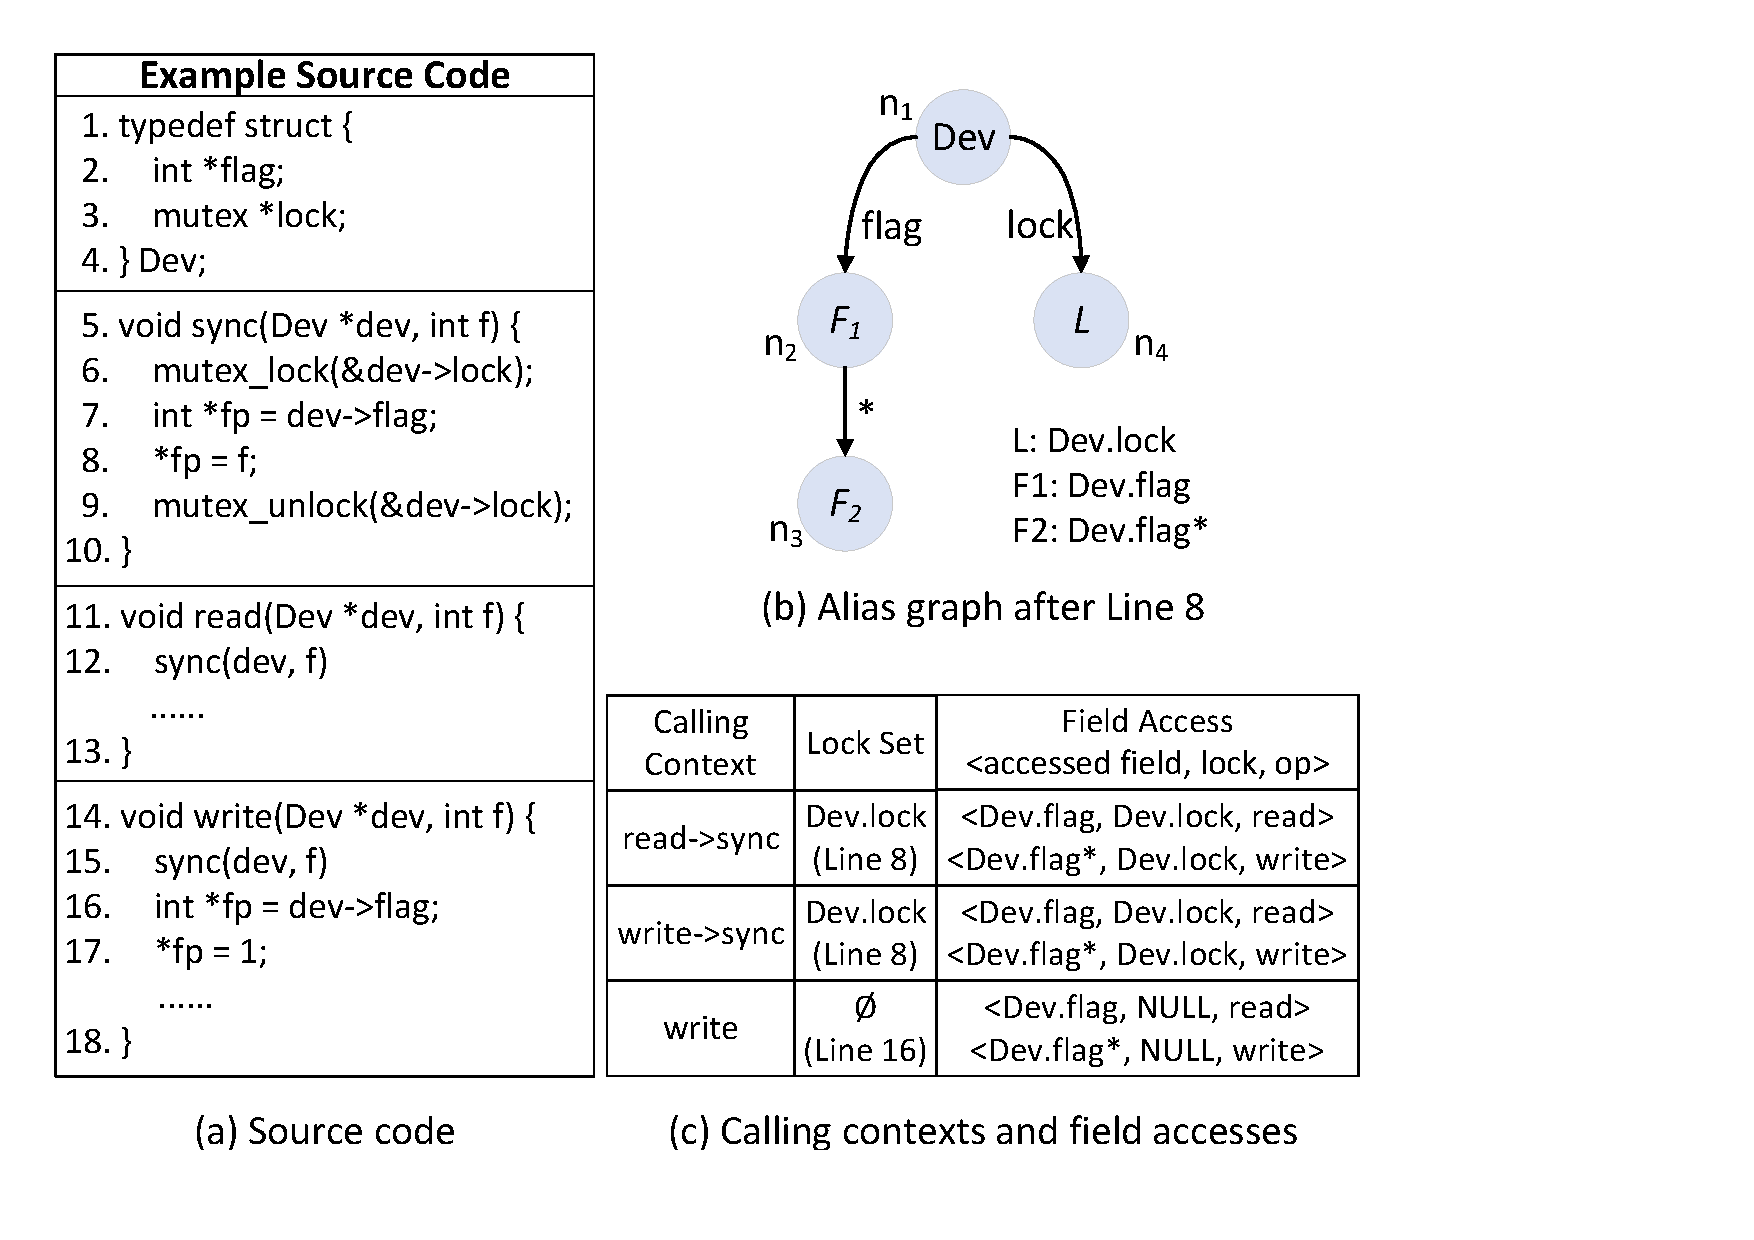
\includegraphics[width=1\linewidth]{figures/fig_demo_rule_mining.pdf}
	\figcaption{Example of locking-rule mining.}
	\label{fig_demo_rule_mining}
\end{figure}

\noindent{\textbf{\em Example.}} We use an example in 
Figure~\ref{fig_demo_rule_mining} to illustrate how to mine locking rules with 
the three stages. The analysis first performs a path-based analysis to extract 
key fields. Take the code path {\tt Line11, Line 12, Line 5, Line 6, Line 7, 
Line 8, Line 9} as an example. The analysis first updates the alias graph by 
handling two GEP operations ({\em \&dev->lock} and {\em fp = dev->flag}) and a 
STORE operation ({\em *fp = f}), and the final alias graph is shown in 
Figure~\ref{fig_demo_rule_mining}(b). And then at the same time as alias 
analysis, the analysis records the acquired lock {\em Dev.lock} into the lock 
set after the lock instruction at Line 6. When analyzing the read instruction 
at Line 7, the analysis finds the node of the accessed field ($\mathit{n_2}$) 
and the node of the lock stored in the lock set ($\mathit{n_4}$) has the same 
ancestor ($\mathit{n_1}$), and thus {\em Dev.flag} is a key field. Similarly, 
{\em Dev.flag*} is also a key field, due to the write instruction at Line 8. 

After extracting key fields, the method collects all accesses to key fields 
with lock-set analysis and the alias graph. Take the code path {\tt Line 14, 
Line 15, Line 5, Line 6, Line 7, Line 8, Line 9, Line 16 and Line 17} as an 
example, through a lock instruction at Line 6, the analysis records the 
acquired lock {\em Dev.lock} into the lock set. When analyzing the read 
instruction at Line 7, the analysis finds the node of the accessed field 
($\mathit{n_2}$) and the node of the lock stored in the lock set 
($\mathit{n_4}$) has the same ancestor ($\mathit{n_1}$), and thus records a 
field access <{\em Dev.flag}, {\em Dev.lock}>. Similar to the read instruction 
at Line 7, the method also records a field access <{\em Dev.flag*}, {\em 
Dev.lock}> for the write instruction at Line 8. Then through an unlock 
operation at Line 9, the analysis removes the lock {\em Dev.lock} from the lock 
set. As a result, the key fields {\em Dev.flag} and {\em Dev.flag*} are 
accessed without acquiring any lock at Lines 16 and 17, and thus the analysis 
records two field accesses <{\em Dev.flag}, {\em NULL}> and <{\em Dev.flag*}, 
{\em NULL}>. The final field accesses are shown in 
Figure~\ref{fig_demo_rule_mining}(c).

After collecting all field accesses, the analysis finds that the fields {\em 
Dev.flag} and {\em Dev.flag*} are accessed under three calling contexts, and 
two of them are protected by the lock {\em Dev.lock}. Besides, there is a write 
to {\em Dev.flag*} at Line 8, and thus the field {\em Dev.flag*} is deduced to 
be protected by the lock {\em Dev.lock} (assume the threshold of the ratio {\em 
locked\_access\_num} / {\em all\_access\_num} is 0.6). However, the access to 
{\em Dev.flag*} at Line 17 is not protected by {\em Dev.lock}, causing a data 
race.

\subsection{Lock-Usage Analysis}
\label{subsec_lock_usage_analysis}
Our analysis takes functions that have no caller function as the entries like 
existing work~\cite{Li:ASPLOS22}, and performs a path-based analysis starting 
from these entry functions. It assumes that all codes reaching from entry 
functions can execute concurrently, to reduce false negatives. However, this 
assumption is too conservative and can introduce many false positives because 
not all entry functions can execute concurrently in fact. We observe that each 
kernel module has an initialization phase, after which many functions can be 
called concurrently by other modules. When performing initialization, the 
kernel module serially initializes the locks and prepares other data for 
subsequent operations. And thus functions with the lock initialization and 
functions called by them tend not to execute concurrently. Based on this 
observation, we propose a lock-usage analysis to filter out false positives 
caused by code that can not execute concurrently.

\begin{figure}[htbp]
	\centering
	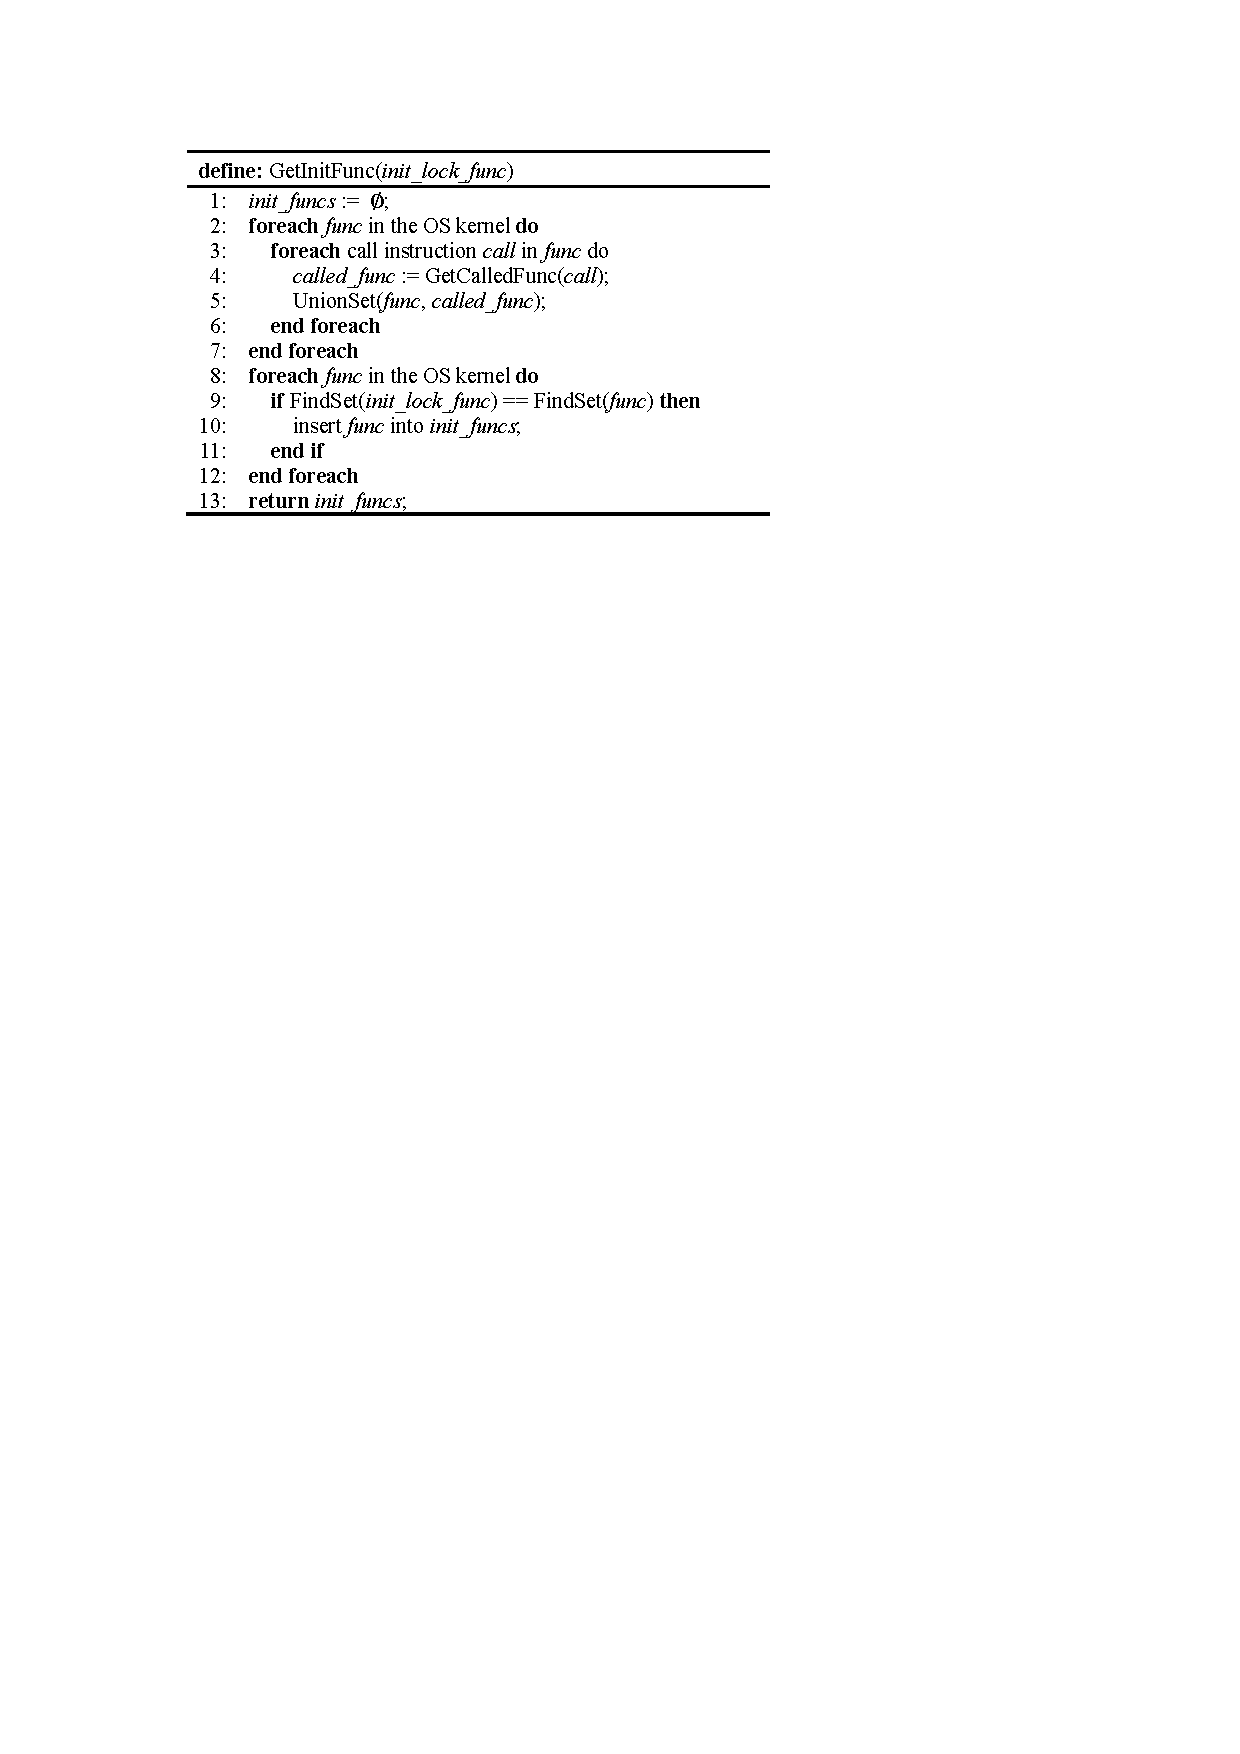
\includegraphics[width=0.9\linewidth]{figures/fig_pseudocode_lock_usage.pdf}
	\figcaption{Pseudocodes of lock-usage analysis.}
	\label{fig_pseudocode_lock_usage}
\end{figure}

Our lock-usage analysis uses the union-find set~\cite{Galler:ACM64} to get all 
functions that are reachable from the lock initialization functions such as 
{\em spin\_lock\_init()} in the function call graph. 
Figure~\ref{fig_pseudocode_lock_usage} shows the pseudocodes of the lock-usage 
analysis. For each analyzed function in the OS kernel, the analysis first gets 
all the called functions of it (Lines 3-4), and then union the analyzed  
function and the called function to update the union-find set (Line 5). After 
processing all the call instructions, the analysis judges whether a function 
executes in the initialization phase by checking whether it exists in the same 
set with the given lock initialization function (Lines 9-11).

\begin{figure}[htbp]
	\centering
	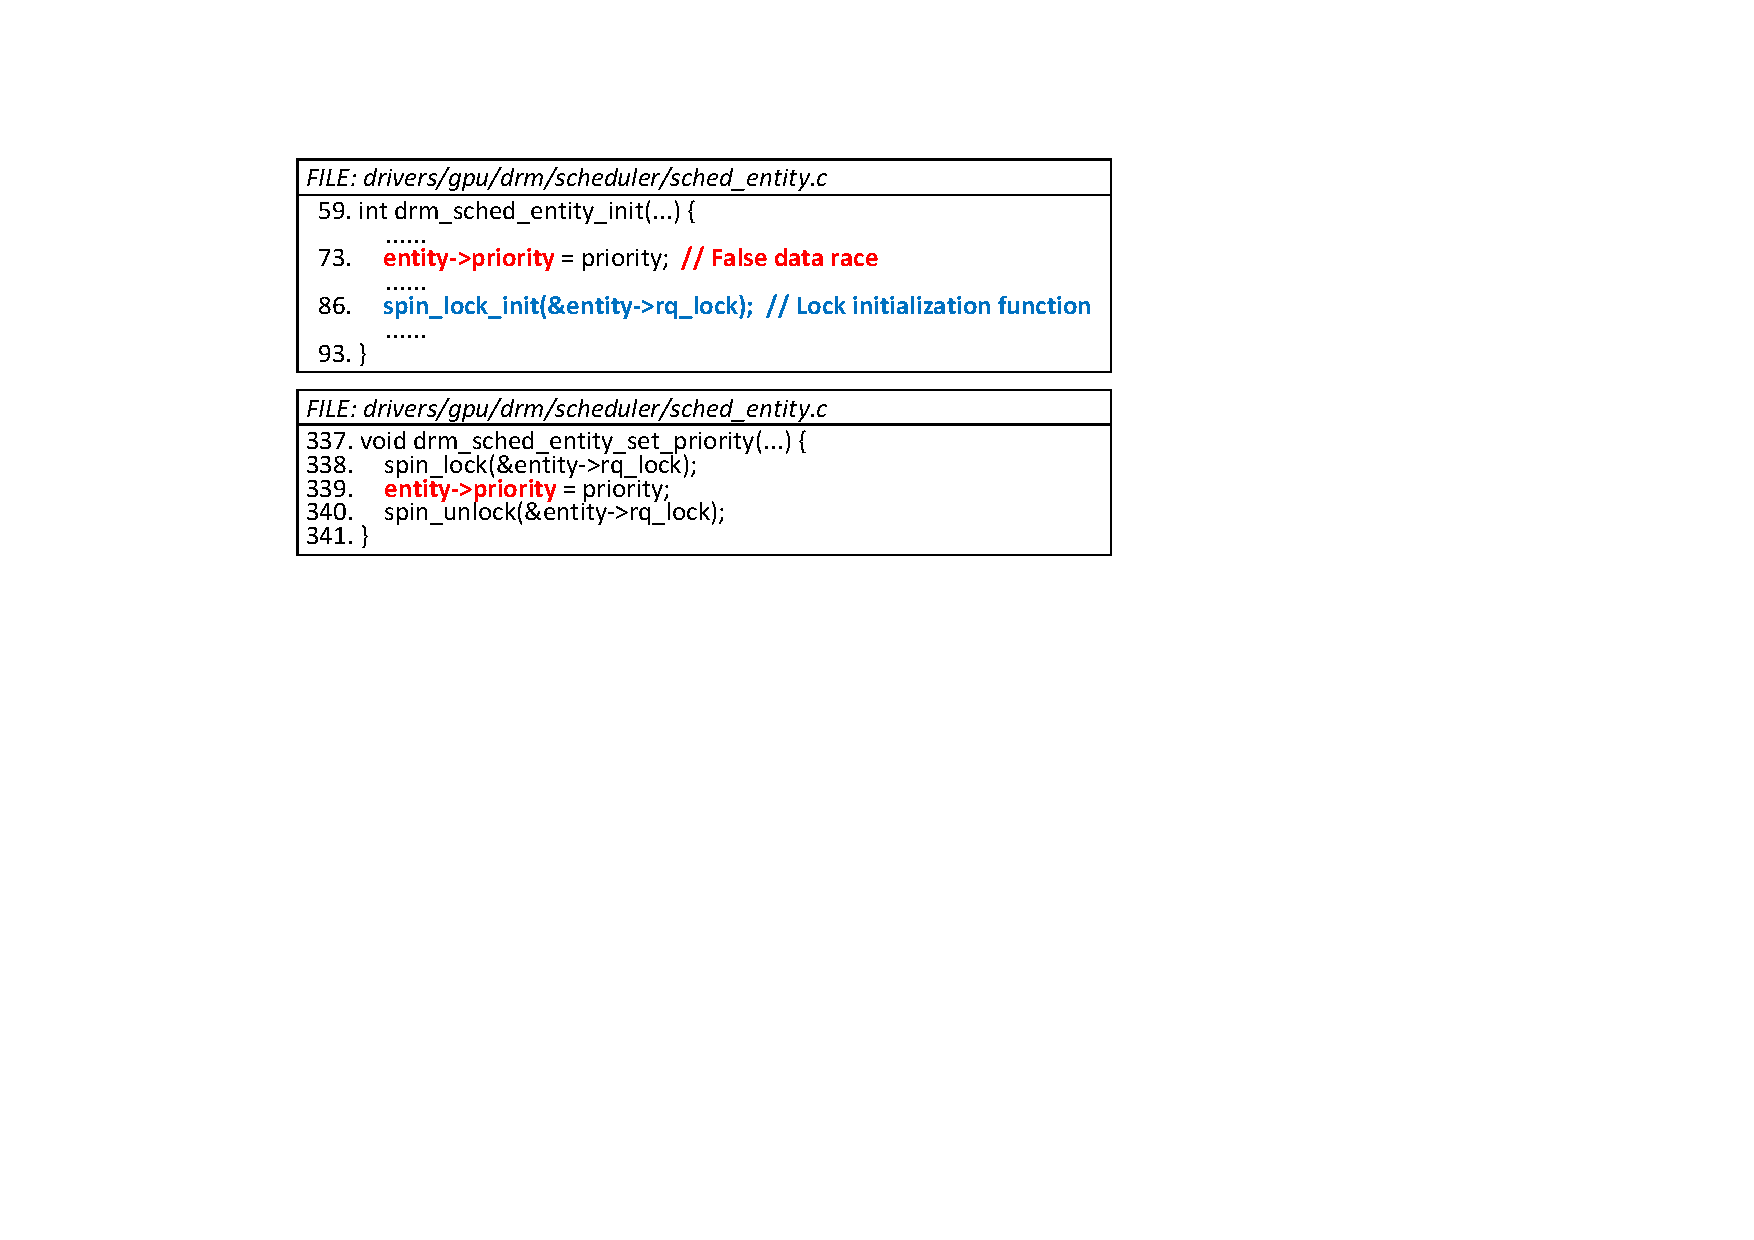
\includegraphics[width=0.9\linewidth]{figures/fig_demo_lock_usage.pdf}
	\figcaption{A false data race filtered out by our lock-usage analysis.}
	\label{fig_demo_lock_usage}
\end{figure}

\noindent{\textbf{\em Example.}} Figure~\ref{fig_demo_lock_usage} shows a false 
data race filtered out by our lock-usage analysis in the Linux DRM scheduler. 
For example in {\em drm\_sched\_entity\_set\_priority()}, the accesses to {\em 
entity->priority} is protected by the lock {\em entity->rq\_lock} in most 
cases. Therefore, {\em entity-priority} is deduced to be protected by the lock 
{\em entity->rq\_lock}. But in {\em drm\_sched\_entity\_init()}, {\em 
entity->priority} is written without acquiring the lock {\em entity->rq\_lock} 
and thus introducing a possible data race. However, the lock initialization 
function {\em spin\_lock\_init()} is called at Line 86 by {\em 
drm\_sched\_entity\_init()}. And thus {\em drm\_sched\_entity\_init()} is 
inferred to execute in the module initialization phase and can not execute 
concurrently with other functions, and this is a false data race.

\subsection{Pattern-Based Estimation}
\label{subsec_estimation}
Many data races are benign or introduced by developers deliberately to improve 
the performance of OS kernels. They can not cause memory or logic bugs in fact, 
and thus developers are unwilling to put effort into repairing them. We observe 
that harmful data races match some typical patterns, and propose a {\em 
pattern-based estimation} to extract data races that can cause memory or logic 
bugs.

At present, we propose three patterns that can cause null-pointer dereference, 
data inconsistencies and double fetches, because these three patterns are 
common and dangerous in OSes. The three patterns are shown in 
Figure~\ref{fig_pattern}, and we assume that accesses to the fields of {\em 
dev} should be protected by {\em dev->lock}.

\begin{figure}[htbp]
	\centering
	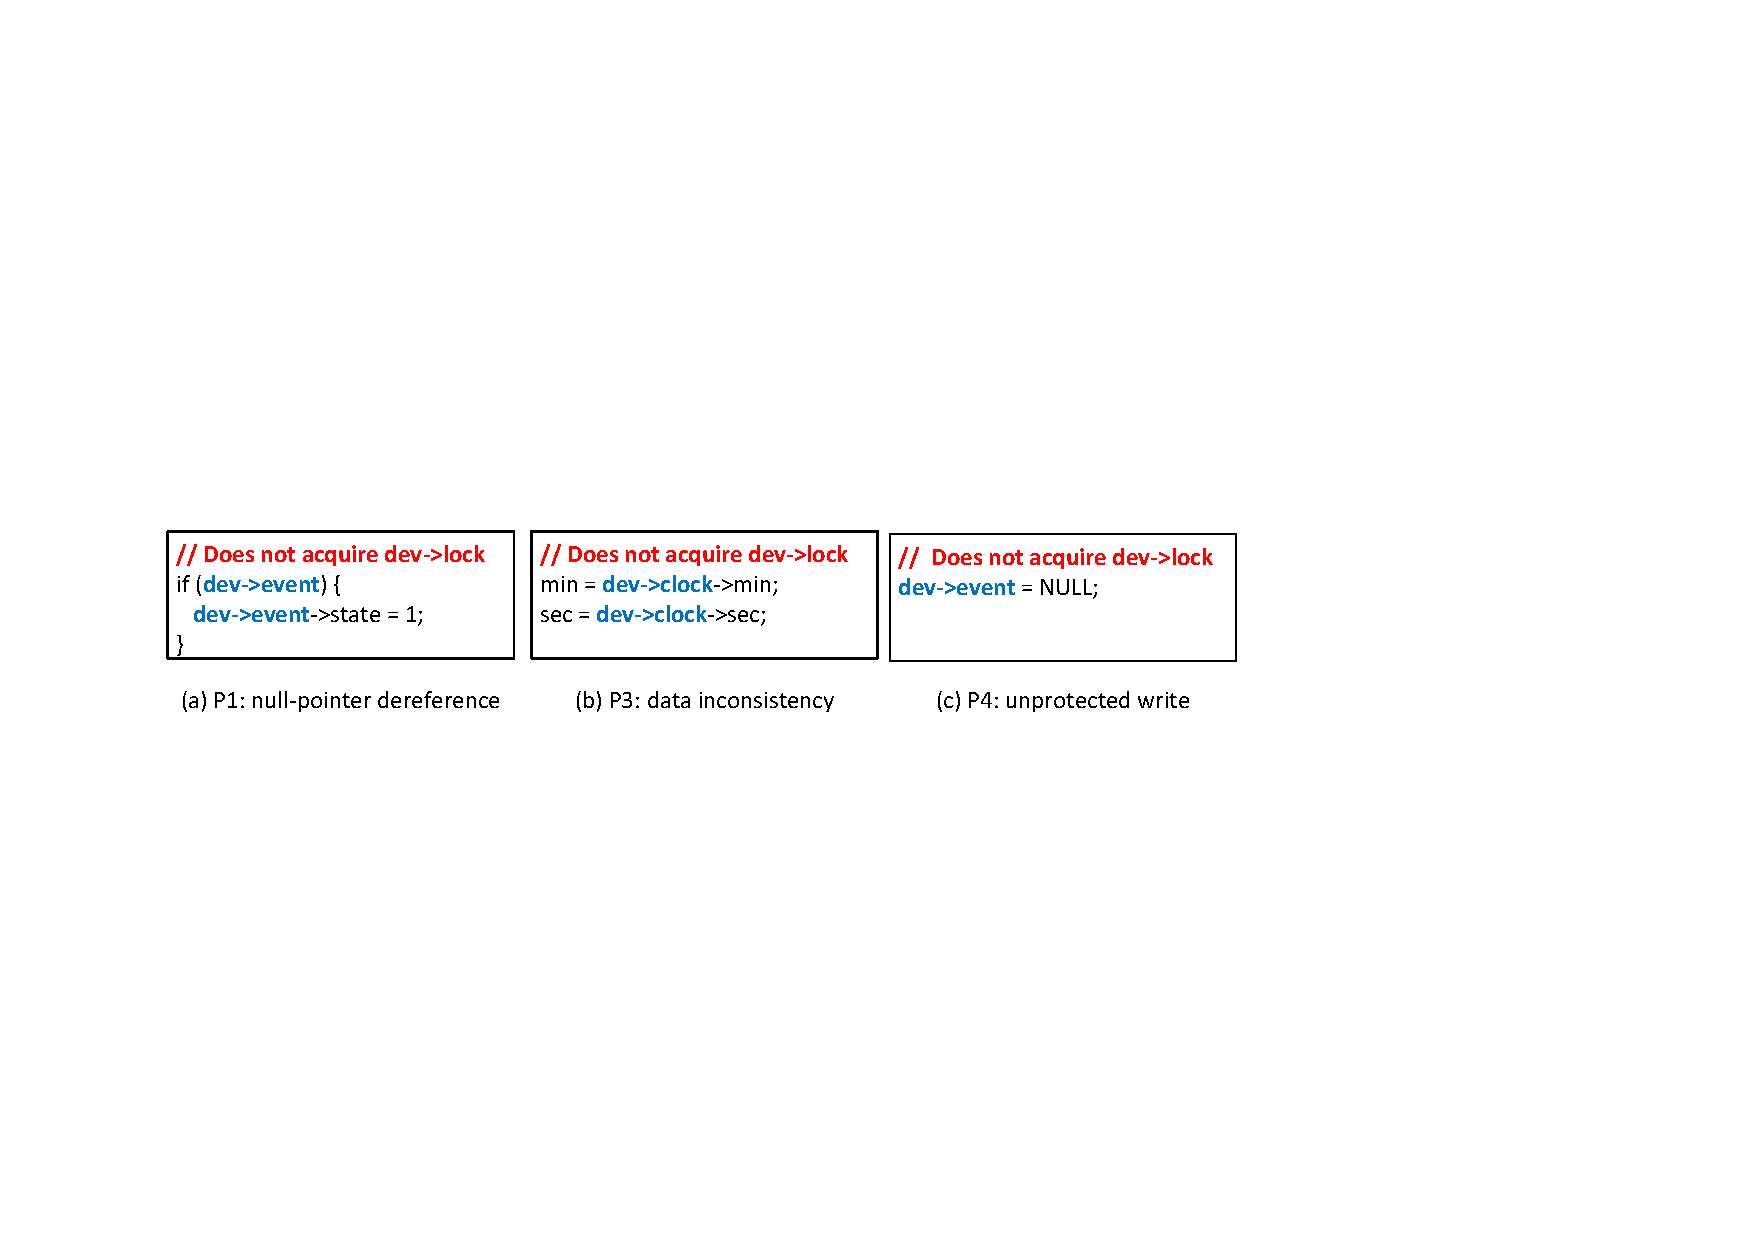
\includegraphics[width=1\linewidth]{figures/fig_pattern.pdf}
	\figcaption{Three harmful patterns of data races.}
	\label{fig_pattern}
\end{figure}

\begin{itemize}
	\item \PP{P1: Null-pointer dereference.} The two accesses to {\em 
	dev->event} 
	are not protected by {\em dev->lock}. This can cause a null-pointer 
	dereference if {\em dev->event} is set to NULL right after the condition of 
	the if statement is checked to be true. To recognize such a pattern, the 
	analysis first locates the data race, if it is checked by an if statement 
	and then dereferenced, a possible null-pointer dereference can occur.
	\item \PP{P2: Data inconsistency.} Two different fields of the same data 
	structure are accessed without acquiring {\em dev->lock}. This can cause a 
	data inconsistency when the data structure field {\em dev->clock} is 
	changed by another thread right after the access to {\em dev->clock->min}. 
	To recognize such a pattern, the analysis detects whether multiple fields 
	of 	the same data structure are accessed without acquiring the protecting 
	lock.
	\item \PP{P3: Double fetch.} The write access to {\em dev->event} is not 	
	protected by {\em dev->lock}. This is dangerous because the value of {\em 	
	dev->event} can be modified at any time when other threads access it. If it 
	is changed during two accesses in another thread, a double fetch can occur, 
	introducing unpredictable behavior. The analysis detects such a pattern by 
	judging whether a data race occurs in a write access.
\end{itemize}
